\documentclass[conference]{IEEEtran}

\usepackage{cite}
\usepackage{amsmath,amssymb}
\usepackage{graphicx}
\usepackage{booktabs}
\usepackage{hyperref}
\usepackage{url}
\usepackage{tikz}
\usetikzlibrary{arrows.meta, positioning}

\title{Report: Emergent Behaviors in Large Language Models}

\author{
\IEEEauthorblockN{Adarsh Kumar Singh\\Ansh Singh}
\IEEEauthorblockA{
Bengaluru, Karnataka, India\\
Email: anshsactivity2024@gmail.com
}
}

\begin{document}

\maketitle

\begin{abstract}
Large language models (LLMs) have demonstrated capabilities that appear unpredictably as model scale increases. These behaviors, commonly referred to as emergent abilities, challenge traditional assumptions about neural network scaling and capability forecasting. This paper surveys current research on emergent behaviors in LLMs, focusing on phenomena such as chain-of-thought reasoning, instruction following, and in-context learning. We review empirical evidence from models including GPT-3, PaLM, and GPT-4 and evaluate competing explanations for emergence. Finally, we discuss implications for AI safety, evaluation methodology, and future research directions.
\end{abstract}

\section{Introduction}

Large language models (LLMs) such as GPT-3, PaLM, and GPT-4 have demonstrated remarkable capabilities across many tasks including reasoning, translation, summarization, and code generation \cite{wei2022emergent}.

The development of models such as GPT-3 demonstrated that increasing model scale can dramatically improve performance across many natural language processing tasks \cite{brown2020gpt3}.

More recent models such as GPT-4 demonstrate further improvements in reasoning, coding, and multimodal capabilities \cite{openai2023gpt4}.

One of the most surprising observations about these models is the appearance of abilities that were not present in smaller models. These capabilities appear suddenly once models reach a certain scale. Researchers refer to these behaviors as \textit{emergent abilities}.

Understanding emergent capabilities is important for several reasons:

\begin{itemize}
\item Understanding how large neural networks learn complex behaviors
\item Predicting future capabilities of increasingly powerful AI systems
\item Ensuring safe deployment of large AI models
\end{itemize}

This report investigates the following questions:

\begin{enumerate}
\item What abilities have been observed to emerge in large language models?
\item What explanations exist for these phenomena?
\item What implications do emergent abilities have for AI safety and governance?
\\
\\
\end{enumerate}
Recent advances in transformer-based architectures have significantly increased the capabilities of machine learning systems. Large language models are trained on massive datasets containing text from books, websites, and other digital sources. As the scale of these models increases, they develop increasingly sophisticated abilities such as reasoning, summarization, translation, and code generation. 

However, researchers have observed that certain capabilities do not appear gradually with model size. Instead, they seem to appear suddenly once models reach specific parameter thresholds. This phenomenon has led researchers to investigate the concept of emergent abilities in neural networks. Understanding why these capabilities arise is an important research problem that combines ideas from machine learning, complex systems, and cognitive science.

\section{Background}
Modern large language models are based on the transformer architecture, which uses attention mechanisms to model relationships between words in a sequence \cite{vaswani2017attention}.
\subsection{Scaling Laws}

Scaling laws describe how the performance of neural networks improves as the size of the model, training data, and computational resources increase. Early empirical studies demonstrated that the loss of language models follows a power-law relationship with model size. This means that performance improves in a predictable way when models become larger.

The Chinchilla scaling law further refined this understanding by showing that optimal performance requires balancing the number of model parameters with the amount of training data. When models are trained with insufficient data relative to their size, performance improvements may plateau.

Although scaling laws generally produce smooth improvements in model performance, researchers have observed that some capabilities appear discontinuously. For example, tasks such as multi-step reasoning or complex arithmetic may show little improvement for smaller models but suddenly improve once the model reaches a certain parameter count. These discontinuities are often interpreted as evidence of emergent abilities in large language models.

\subsection{Emergent Abilities}

Wei et al. define emergent abilities as capabilities that are not present in smaller models but appear in larger models \cite{wei2022emergent}. Examples include reasoning, instruction following, and multi-step problem solving.
The concept of emergence originates from complex systems theory, where new behaviors appear when a system becomes sufficiently large or complex. In the context of large language models, emergence refers to the appearance of capabilities that cannot easily be predicted from the behavior of smaller models.

Researchers have identified a wide variety of emergent behaviors across different tasks. These include symbolic reasoning, mathematical problem solving, code synthesis, and instruction following. The appearance of these abilities suggests that large neural networks may internally develop representations that support increasingly complex forms of reasoning.
The BIG-Bench benchmark was developed to evaluate emergent capabilities across a diverse set of challenging tasks \cite{srivastava2022bigbench}.

Understanding these emergent behaviors is crucial for both scientific and practical reasons. From a scientific perspective, studying emergence can help researchers understand how neural networks process information and learn abstract concepts. From a practical perspective, identifying when new capabilities appear can help developers anticipate the behavior of future AI systems.

\subsection{In-Context Learning}

Large language models can learn tasks directly from examples provided in prompts. This phenomenon, called in-context learning, enables models to perform tasks without updating model parameters.

However, some researchers argue that many emergent abilities may actually reflect improvements in in-context learning rather than new reasoning capabilities \cite{prasad2023icl}.

\section{Conceptual Model of Emergence}

Figure \ref{fig:emergence_diagram} illustrates a conceptual explanation of how emergent abilities may arise as models scale.

\begin{figure}[h]
\centering
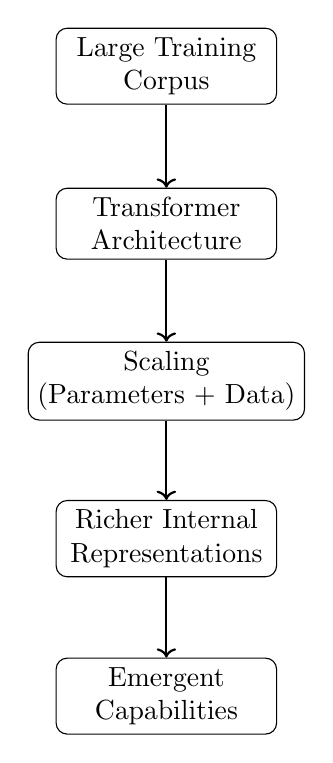
\begin{tikzpicture}[
node distance=2cm,
box/.style={rectangle, draw, rounded corners, minimum width=2.8cm, minimum height=0.9cm, align=center},
arrow/.style={->, thick}
]

\node[box] (data) {Large Training\\Corpus};
\node[box, below of=data] (model) {Transformer\\Architecture};
\node[box, below of=model] (scale) {Scaling\\(Parameters + Data)};
\node[box, below of=scale] (represent) {Richer Internal\\Representations};
\node[box, below of=represent] (emerge) {Emergent\\Capabilities};

\draw[arrow] (data) -- (model);
\draw[arrow] (model) -- (scale);
\draw[arrow] (scale) -- (represent);
\draw[arrow] (represent) -- (emerge);

\end{tikzpicture}

\caption{Conceptual illustration of emergent capability formation in large language models.}
\label{fig:emergence_diagram}
\end{figure}

\section{Chain-of-Thought Reasoning}

Chain-of-thought prompting enables models to generate intermediate reasoning steps before producing a final answer \cite{wei2022cot}.

\begin{figure}[h]
\centering
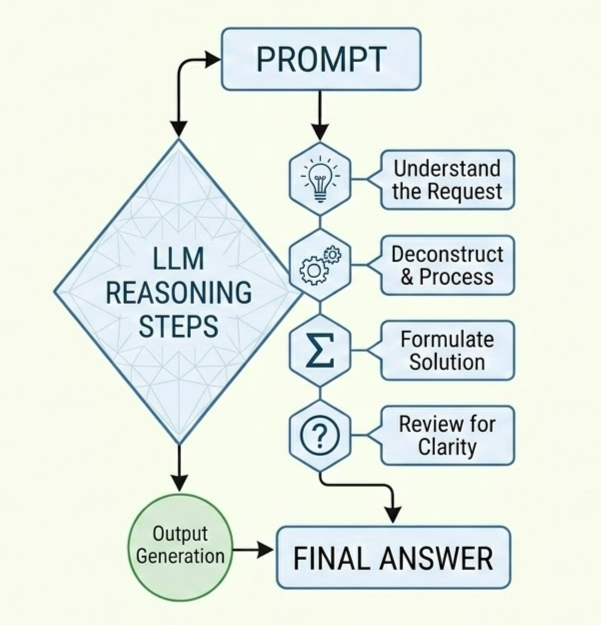
\includegraphics[width=0.45\textwidth]{cot.png}
\caption{Illustration of chain-of-thought prompting where models generate intermediate reasoning steps.}
\label{fig:cot}
\end{figure}

Experiments show that chain-of-thought reasoning emerges primarily in models larger than approximately 100 billion parameters.

Chain-of-thought prompting has become an important technique for improving reasoning performance in large language models. By encouraging the model to generate intermediate reasoning steps, the prompt effectively guides the model through a structured reasoning process.

Research has shown that chain-of-thought prompting significantly improves performance on tasks such as arithmetic reasoning, commonsense reasoning, and symbolic logic. Interestingly, the effectiveness of this prompting technique strongly depends on model size. Smaller models often fail to produce coherent reasoning steps, while larger models generate structured and logically consistent explanations.

This observation provides strong evidence for the existence of emergent reasoning abilities. Once models reach a sufficient scale, they appear capable of internally representing multi-step reasoning processes that were not present in smaller models.

\section{Empirical Evidence}

\begin{table}[h]
\centering
\begin{tabular}{lll}
\toprule
Capability & Threshold & Example Models \\
\midrule
Few-shot arithmetic & $\sim$13B & GPT-3, PaLM \\
Word unscrambling & $\sim$52B & BIG-Bench models \\
Chain-of-thought reasoning & $\sim$100B & GPT-3, PaLM \\
Multilingual reasoning & $\sim$62B & PaLM \\
Code generation & $\sim$10B & Codex, GPT-4 \\
Instruction following & 6--13B & InstructGPT \\
\bottomrule
\end{tabular}
\caption{Examples of emergent capabilities in LLMs}
\end{table}
The empirical observations summarized in Table I suggest that different capabilities emerge at different model sizes. Simpler abilities such as instruction following appear at relatively small scales, while more complex reasoning abilities require significantly larger models.

Large models such as PaLM demonstrated strong performance on reasoning tasks including arithmetic and commonsense reasoning \cite{chowdhery2022palm}.

For example, code generation capabilities have been observed in models with approximately ten billion parameters, whereas advanced reasoning techniques such as chain-of-thought prompting tend to appear in models with over one hundred billion parameters. These differences suggest that emergent abilities may depend on the complexity of the internal representations required for each task.

Furthermore, experiments across multiple model families indicate that these trends are consistent across different architectures. This suggests that emergence is not limited to a single model design but may instead be a general property of large neural networks.

\begin{figure}[h]
\centering
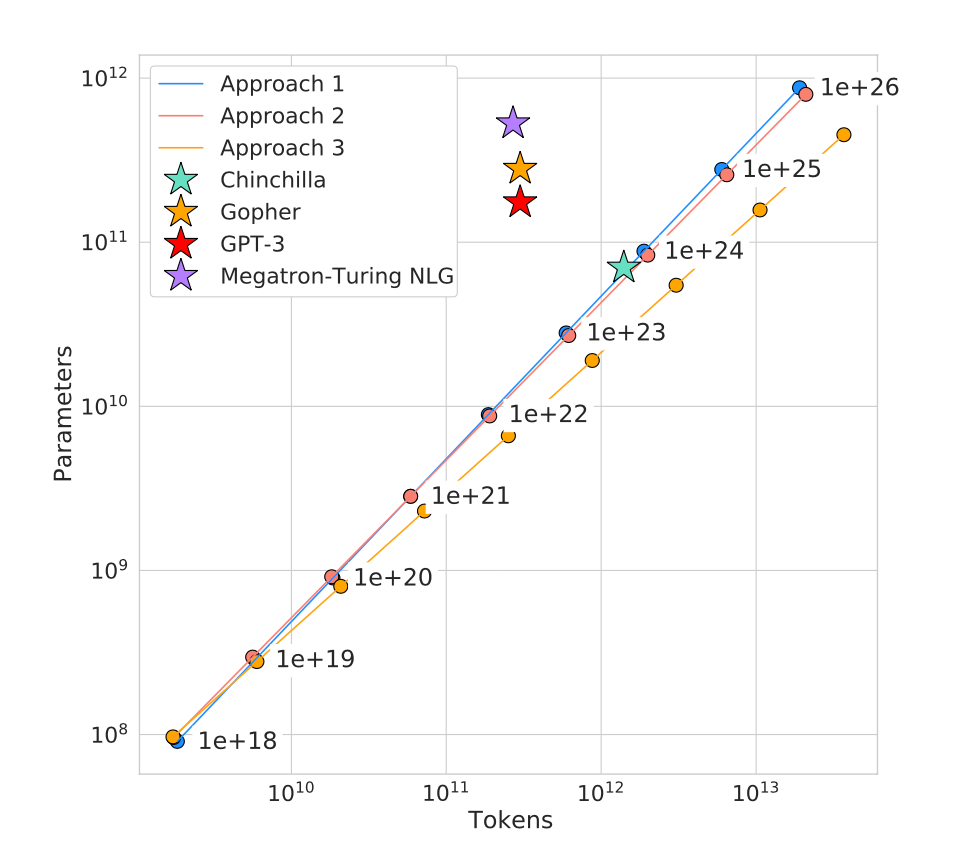
\includegraphics[width=0.45\textwidth]{Scaling.png}
\caption{Example scaling curve showing performance improvement with increasing model size.}
\label{fig:scaling}
\end{figure}

\section{Emergent Capabilities vs Model Size}

\begin{figure}[h]
\centering
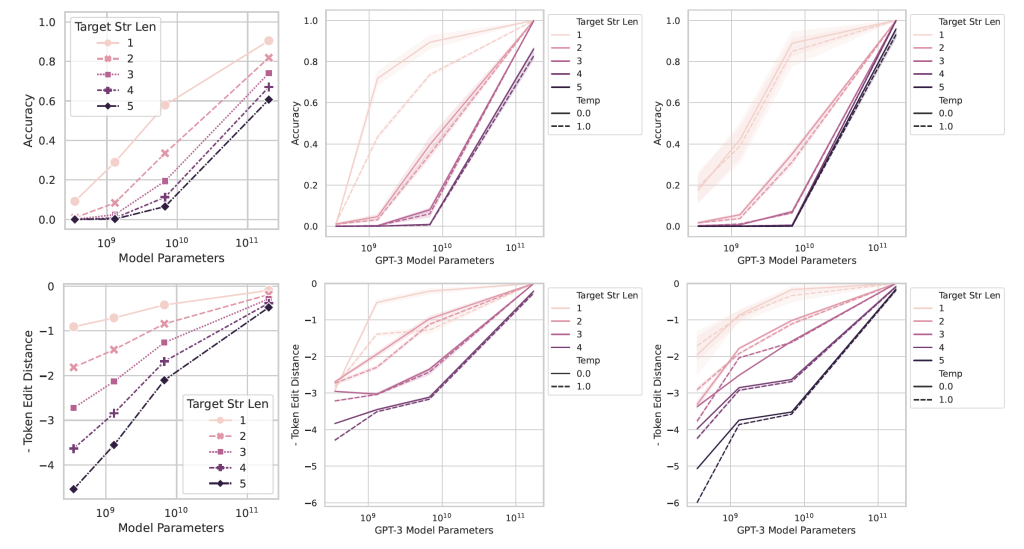
\includegraphics[width=0.45\textwidth]{emergent_capabilities.png}
\caption{Different capabilities emerge at different model scales.}
\label{fig:capabilities}
\end{figure}

\section{Competing Theories}

\subsection{Phase Transition Hypothesis}

Some researchers propose that emergent abilities correspond to phase transitions in neural representations \cite{wei2022emergent}.

\subsection{In-Context Learning Explanation}

Others argue emergence reflects improved prompt interpretation and generalization ability \cite{prasad2023icl}.

\subsection{Metric Artifacts}

Another explanation suggests that evaluation metrics may create artificial discontinuities in performance curves \cite{schaeffer2023emergent}.

\section{Safety Implications}

Emergent capabilities introduce uncertainty in predicting AI behavior. Potential risks include misuse for cyberattacks, misinformation, or autonomous decision-making.

Ensuring that increasingly powerful AI systems behave safely and reliably is an important challenge for the research community \cite{christiano2017rlhf}.

Mitigation strategies include:

\begin{itemize}
\item extensive model evaluation
\item adversarial testing
\item staged deployment
\item capability-based regulation
\end{itemize}

The unpredictability of emergent abilities presents significant challenges for AI safety and governance. If new capabilities appear suddenly at larger model scales, it may be difficult for developers and policymakers to anticipate the behavior of future AI systems.

For example, advanced reasoning capabilities could enable models to perform tasks that were not explicitly intended by their designers. In some cases, these capabilities could be misused for harmful purposes such as generating misinformation, automating cyberattacks, or manipulating users.

As a result, researchers have proposed developing more rigorous evaluation frameworks for large AI systems. These frameworks aim to detect potentially dangerous capabilities before models are deployed in real-world applications. Improving transparency and interpretability of neural networks will also be important for managing the risks associated with emergent AI capabilities.
\section{Future Research}

Important research directions include mechanistic interpretability, theoretical explanations of emergence, and studying emergent behavior in multimodal models.
\subsection{Mechanistic Interpretability}

One promising research direction is mechanistic interpretability, which aims to understand how neural networks internally represent information. By studying the internal structure of large language models, researchers may be able to identify the mechanisms responsible for emergent reasoning abilities.

\subsection{Predicting Emergent Abilities}

Another important research goal is developing methods to predict when emergent abilities will appear. If researchers can identify reliable indicators of emergence, it may become possible to forecast the capabilities of future models before they are fully trained.

\subsection{Multimodal Emergence}

Future AI systems increasingly combine multiple modalities such as text, images, audio, and video. Studying emergent behaviors in these multimodal models will be an important step toward understanding the broader phenomenon of emergence in artificial intelligence.

\section{Case Study: Emergence of Reasoning in GPT-3 vs GPT-4}

To better understand emergent abilities, it is useful to examine how reasoning capabilities evolved across different generations of large language models. In this section we compare reasoning performance between GPT-3 and GPT-4 using results reported in recent research.

GPT-3, released in 2020, contains approximately 175 billion parameters and demonstrated strong performance on many natural language processing tasks \cite{brown2020gpt3}. However, while GPT-3 could perform simple reasoning tasks, it often struggled with complex multi-step problems that required structured reasoning.

For example, when asked to solve multi-step arithmetic or logical reasoning problems, GPT-3 frequently produced incorrect answers or incomplete reasoning chains. Researchers discovered that providing explicit reasoning steps in prompts could significantly improve performance. This technique later became known as chain-of-thought prompting \cite{wei2022cot}.

In contrast, newer models such as GPT-4 demonstrate significantly stronger reasoning abilities. GPT-4 is capable of solving more complex tasks involving multi-step reasoning, code generation, and structured problem solving \cite{openai2023gpt4}. These improvements suggest that larger models may internally develop representations that support more advanced reasoning processes.

One explanation for this improvement is that larger models learn richer internal representations of language and knowledge during training. As the number of parameters increases, the model may develop internal structures that allow it to perform more complex reasoning operations.

\begin{table}[h]
\centering
\begin{tabular}{lll}
\toprule
Model & Parameters & Key Abilities \\
\midrule
GPT-3 & 175B & Few-shot learning, basic reasoning \\
PaLM & 540B & Improved reasoning, multilingual tasks \\
GPT-4 & Unknown & Advanced reasoning, coding, multimodal tasks \\
\bottomrule
\end{tabular}
\caption{Comparison of capabilities across major large language models}
\end{table}

This comparison between GPT-3 and GPT-4 illustrates the concept of emergent capabilities. While smaller models may show limited reasoning abilities, larger models often demonstrate qualitatively different behaviors once they reach a sufficient scale. Understanding these transitions remains an important challenge for researchers studying large language models.

\section{Conclusion}

Emergent abilities represent one of the most intriguing phenomena observed in modern artificial intelligence systems. As large language models continue to grow in scale, they demonstrate increasingly complex behaviors that were not present in earlier generations of models.

While researchers have proposed several explanations for these behaviors, including phase transitions, improved in-context learning, and evaluation artifacts, the precise mechanisms underlying emergence remain an open question. Continued research will be necessary to fully understand how neural networks develop these capabilities.

Understanding emergent behaviors will be essential for guiding the safe development of future AI systems. By improving our ability to analyze and predict emergent capabilities, researchers can ensure that increasingly powerful models are deployed responsibly and beneficially.

\bibliographystyle{IEEEtran}
\bibliography{references}

\end{document}